% -*- root: ../../../main.tex -*-
\subsection{Safety e Consistency}
Nelle sezioni precedenti è stato descritto il funzionamento generale di RAFT includendo alcune proprietà e vincoli essenziali per mantenere consistenza tra i log durante le principali operazioni.\\
Qui di seguito ricordiamo le proprietà nominate nelle sezioni precedenti:

\begin{itemize}
	\item{\textbf{Election Safety:}} 
  Per un dato term è possibile al più eleggere \textbf{un solo leader}.
	La dimostrazione di questa proprietà è già stata discussa precedentemente nella sezione \ref{electionsaf}.
	\item{\textbf{Leader Append-Only:}}
  Il leader non cancella \textbf{mai}, ne sovrascrive le entry del proprio log.
  La proprietà è descritta in dettaglio nella sezione \ref{Log Replication}.
	\item{\textbf{Log Matching:}}
  La proprietà di log matching garantisce che:
	\begin{itemize}
		\item{\emph{Se due log hanno un entry con lo stesso index e stesso term, allora quell'entry contiene lo stesso comando(sono identiche)}}.
		\item{\emph{Se due \textit{entry} in log diversi hanno lo stesso index e lo stesso term, allora anche tutte le loro precedenti entry sono identiche tra i due log}}.
	\end{itemize}
	La proprietà è descritta in dettaglio nella sezione \ref{Log Matching}.
\end{itemize}
L'elenco sovrastante non è però completo! Attualmente ci sono casi che non sono gestiti e che possono causare notevole \textbf{inconsistenza} tra i log.\\
Ad esempio se il leader \textit{valida} alcune \textit{entry} mentre un dato follower è offline, nel caso in cui il follower venisse eletto esso potrebbe sovrascrivere le entry gia eseguite con quelle presenti nel proprio log.\\
E' necessario dunque completare l'algoritmo aggiungendo la proprietà chiave di tutte le state machine, la \textbf{State Machine Safety} property. 

  \paragraph{State Machine Safety}
  \emph{Non appena una entry è stata committata ed eseguita in una state machine, allora nessun altra state machine può committare una valore differente per la stessa entry}.\\
  la state machine safety porta all'introduzione di due \textbf{restrizioni} molto importanti all'algoritmo:
  \begin{itemize}
    \item{\textbf{Restrizione durante la leader election}}
    \item{\textbf{Restrizione nei commitment}}
  \end{itemize}


  \subsubsection{Restrizioni nelle Elezioni}
  Durante le elezioni ci sono casi in cui non è possibile determinare se un \textit{entry} è committed oppure no. Come si può vedere in figura \ref{fig:figure10} non è possibile determinare se l'ultima \textit{entry} è stata committed: per questo si aggiunge un \textbf{ulteriore vincolo all'elezione di un candidate}.
  \[
    \emph{\textbf{Scegli il candidato con il log più completo.}}
  \]

  Più precisamente il candidate invia solo le informazioni sull'\textbf{ultima entry} dato che queste informazioni definisco interamente il log.
 \[
      AppendEntries(term, index)
  \]
  Il criterio con cui viene fatta questa valutazione è il seguente:\\
  Sia $lastTerm_v$ il term presente a indice $lastIndex_V$ della entry del log del \textbf{server votante} e $lastTerm_c$ il term presente a indice $lastIndex_C$ della entry del log del \textbf{candidate}, Allora:
  \begin{equation} \label{eq:1}
    \begin{multlined}
    Se:\\
      (lastTerm_v > lastTerm_c) \; \| \;        \\
      (lastTerm_v == lastTerm_c)  \; \&\& \;
      (lastIndex_v > lastIndex_c)
    \implies Reject
    \end{multlined}
  \end{equation}
  In altre parole:
  \begin{itemize}
    \item{\emph{Se l'ultimo term del log del server votante è maggiore di quello del server candidato, allora la  richiesta viene rifiutata. }}
    \item{\emph{Se invece i due ultimi term si equivalgono, la valutazione viene fatta tenendo conto della lunghezza del log:}}
    \begin{itemize}
      \item{\emph{Se l'ultimo indice del log di C è maggiore di quello di V la richiesta viene accettata, altrimenti viene rifiutata.}}
    \end{itemize}
  \end{itemize}
 
  \begin{figure}[H]
  	\centering
  	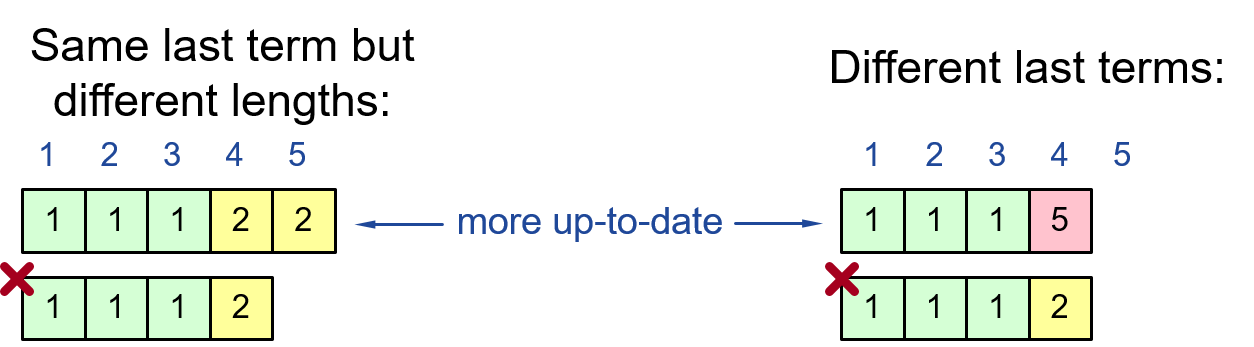
\includegraphics[width=0.99\columnwidth]{raft/pickingUpToDateLeader}
  	\captionsetup{singlelinecheck=off}
  	\caption[stateDiagramCaption]{
	 In questo caso non è possibile determinare se l'ultima \textit{entry} è validata, inoltre solo il primo server può essere eletto dato che il terzo non è disponibile.}
  	\label{fig:figure10}
  \end{figure}

  \paragraph{Commiting di Entries del term corrente}
  Vediamo ora un esempio di quello che è stato detto fino ad ora. Nella figura \ref{fig:figure11} possiamo vedere che all'indice 4 il leader $S1$ al term 2 è riuscito a \textbf{replicare con successo} la propria entry sulla maggioranza dei server; la entry è dunque \textbf{committed}. A questo punto nel caso in cui il leader $S1$ crashasse, per l'\textbf{election restriction} introdotta sopra, i server $S4$ e $S5$ non potrebbero essere eletti leader!\\
  $S5$ non può essere eletto perché non possiede un term più piccolo di tutti gli altri $\rightarrow$ \textbf{condizione n:1}\\
  $S4$ non può essere eletto poiché anche se possiede un term aggiornato non ha un log completo (più corto) $\rightarrow$ \textbf{condizione n:2} 

  \begin{figure}[H]
    \centering
    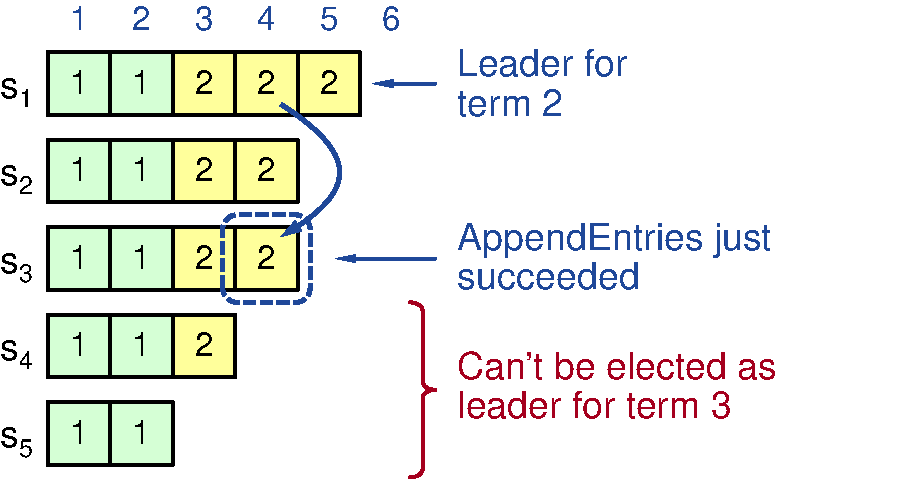
\includegraphics[width=0.99\columnwidth]{raft/committingEntryFromCurrentTerm}
    \caption[stateDiagramCaption]{$S4$ e $S5$ si trovano impossibilitati ad essere eletti come leader e quindi non sono in grado di modificare il log di latri server.}
    \label{fig:figure11}
  \end{figure}

  \subsubsection{Committing di Entries di term precedenti}
  Questo caso, rappresentato perfettamente nell'immagine \ref{fig:figure12} rappresenta la situazione peggiore e più inusuale per RAFT; essa si può riassumere come segue:
  \begin{enumerate}
    \item{Il server $S1$, leader al \textbf{term 2}, \textbf{replica la entry} solamente su due server e poi crasha}
    \item{Un altro server, $S5$ viene eletto leader per il \textbf{term 3} da $S3$ $S4$ $S5$, esso appende una serie di entry e poi crasha prima di poter comunicare.}
    \item{Il server $S1$ si risveglia e viene eletto leader da $S1$ $S2$ $S3$ $S4$, e prima di tutto cerca di \textbf{riparare} il log del sever $S3$ inviando la entry mancante.}
    \item{Il server $S5$ quando riceve gli \textbf{ack} da parte dei followers però \textbf{NON COMMITTA!}}
    \item{Se infatti \textbf{$S1$ crashasse dopo aver committato la entry 3} allora $S5$ può essere eletto, soddisfa entrambi i casi di \ref{eq:1}}
    \begin{itemize}
      \item{\textbf{Caso A}}
      \[
        lastTerm_{S5} > lastTerm_{Si} \qquad \forall i \in [2,3,4]
      \]
      \item{\textbf{Caso B}}
      \[
        lastIndex_{S5} > lastIndex_{Si} \qquad \forall i \in [2,3,4]
      \]
    \end{itemize}
    \item{Se $S5$ venisse eletto al \textbf{term 5} cercherebbe di propagare il proprio log e questo \textbf{obbligherebbe $s1$ $S2$ $S3$ $S4$ a dover riscrivere i propri log}.\\
    \textbf{NB:} Qua abbiamo una totale mancanza di safety, infatti \emph{$S1$ non saprebbe cosa fare dato che una volta commitati i log non possono essere cancellati}}.
  \end{enumerate}
  \begin{figure}[H]
    \centering
    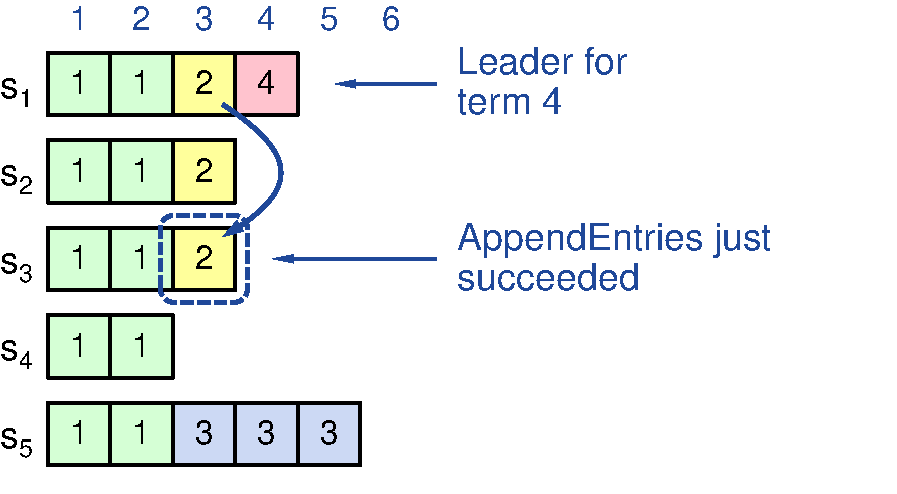
\includegraphics[width=0.99\columnwidth]{raft/committingEntryFromEarlierTerm}
    \caption[stateDiagramCaption]{}
    \label{fig:figure12}
  \end{figure}
  \paragraph{Soluzione:}
  Le regole di committing vengono estese al fine di garantire safety. Ogni leader decidere se una entry è da committare in base a queste regole:
  \begin{itemize}
    \item{\emph{\textbf{La entry deve essere presente nella maggioranza dei server}}}
    \item{\emph{\textbf{Almeno una nuova entry proveniente dal leader dell'attuale term deve essere presente nella maggioranza dei server}}}
  \end{itemize}
  Come vediamo in figura \ref{fig:figure13}, nel momento in cui $S1$ viene eletto leader per il \textbf{term 4} e riesce a replicare la entry sulla maggioranza dei servers allora può finalmente \textbf{propagare le informazioni di committment} riferite a term passati.\\
  Questo garantisce che il server $S5$ non possa essere eletto leader al \textbf{term 5} per la regola 1 in \ref{eq:1}.
  \begin{figure}[H]
    \centering
    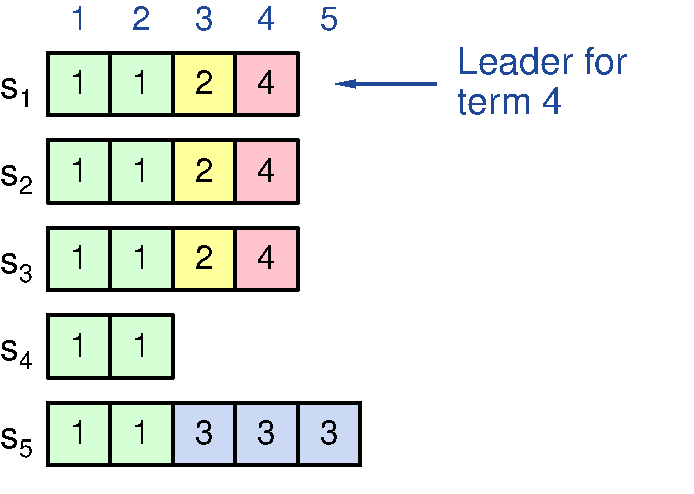
\includegraphics[width=0.80\columnwidth]{raft/newCommitmentRules}
    \caption[stateDiagramCaption]{Quando $S4$ diviene leader non committa immediatamente le entry passate ma attende l'arrivo di nuove entry. Questo evita che $S5$ possa diventare leader sovrascrivendo i logs e portando inconsistenze.}
    \label{fig:figure13}
  \end{figure}
  \subsubsection{Neutralizzazione di vecchi leader}
  Supponiamo che un leader venga momentaneamente disconnesso dalla rete, creando una cosiddetta \textbf{network partition}. RAFT essendo un algoritmo che soddisfa il requisito di \textbf{partition tolerance} garantisce che il cluster sopravviva alla failure di un membro; il cluster semplicemente eleggerà un nuovo leader.\\
  \emph{Cosa succede però se il vecchio leader torna in campo e decide di continuare a governare?}\\
  Per evitare inconsistenze RAFT mette in pratica un comportamento molto semplice, chiamato \textbf{Neutralization of stale leader}, esso funziona in modo molto semplice:
  \begin{itemize}
    \item{Ogni messaggio scambiato contiene al suo interno il \textbf{term del mittente}}.
    \item{\textbf{Caso A}}
      \[
        senderTerm > receiverTerm
      \]
      \begin{itemize}
        \item{\textbf{Il messaggio viene rifiutato.}}
        \item{\textbf{Il mittente si converte a follower.}}
      \end{itemize}
      \item{\textbf{Caso B}}
      \[
        receipTerm > senderTerm
      \]
      \begin{itemize}
        \item{\textbf{Il ricevente si converte a follower.}}
        \item{\textbf{Il ricevente aggiorna il suo term a l'ultimo ricevuto.}}
        \item{\textbf{Il ricevente processa il messaggio normalmente.}}
      \end{itemize}
  \end{itemize}
  Seguendo questi semplici casi, una volta che una \textbf{lezione} per un nuovo leader è \textbf{terminata} non è possibile che un leader deposto possa inviare messaggi alla maggioranza del cluster poiché tale maggioranza possiederà un \textbf{term aggiornato dall'ultima elezione}.